\documentclass[14pt,a4paper]{article}
\usepackage{mathtools}
\usepackage{amsmath}
\usepackage{amsthm}
\setcounter{MaxMatrixCols}{20}
\usepackage{mathrsfs}
\usepackage{setspace}
\usepackage{amsfonts}
\usepackage{geometry}
\geometry{a4paper, total = {210mm,297mm},left=25mm, right=20mm,top=25mm,bottom=25mm}
\usepackage{xcolor}
\usepackage{mcode}
\usepackage{listings}
\lstset{basicstyle = \fontsize{11}{12} \selectfont\ttfamily}
\usepackage{graphicx}


%Begin document - Numerical Analysis - Homework 6

\begin{document}
\label{cover}
\begin{center}
	\vspace*{3cm}
	\large{\textbf{MATH/CS 5466 NUMERICAL ANALYSIS \\ Homework 6}}
	\vfill
	\textbf{Luan Cong Doan} \\ luandoan@vt.edu
	%\vfill
%	Department of Mechanical Engineering \\ Virginia Polytechnic Institute and State University
	\vfill
	\today
\end{center}
\pagebreak

\label{Answer Sheet - Numerical Homework 6}
\doublespacing

\label{Problem 1}
\large\textbf{Problem 1.} Consider the differential equation $x'(t) = \lambda x(t)$ with $x(0) = x_0$.
\begin{enumerate}
	\label{1a}
	\item Show that when applied to this equation, Heun's method yields:\\
	\hspace*{5cm} $x_{k+1} = (1+h\lambda + \frac{1}{2}h^2\lambda^2)x_k$\\
	For Heun's method: $x_{k+1} = x_k + \dfrac{h}{2}(K_1 + K_2)$ with:\\  % + \dfrac{h}{2}, x_k + \dfrac{h}{2}f(t_k,x_k)\right)$\\
	\hspace*{1cm} $K_1 = K_1(t,x) = f(t_k,x_k) = \lambda x_k$\\
	\hspace*{1cm} $K_2 = K_2(t,x;h) = f(t_k+h,x_k+hK_1) = \lambda(x_k + \lambda hx_k)$\\
	$\Rightarrow x_{k+1} = x_k + \dfrac{h}{2}\left( \lambda x_k + \lambda x_k + \lambda^2 hx_k \right) = x_k + \lambda hx_k + \dfrac{h^2}{2}\lambda^2x_k = \left( 1+ h\lambda + \dfrac{1}{2}h^2\lambda^2\right)x_k$
	
	\label{1b}
	\item Develop and analogue of the formula for $x_{k+1}$ in part (a), but now using the four-stage Runge-Kutta method.\\
	The classical 4th-order Runge-Kutta method is: $x_{k+1} = x_k + \frac{1}{6}h(K_1 + 2K_2 + 2K_3 + K_4)$\\
	In our case:\\
	$K_1 = f(t_k,x_k) = \lambda x_k$\\
	$K_2 = f(t_k+\frac{1}{2}h,x_k+\frac{1}{2}hK_1) = \lambda(x_k + \frac{1}{2}\lambda hx_k) = \lambda x_k + \frac{1}{2}\lambda^2hx_k$\\
	$K_3 = f(t_k+\frac{1}{2}h,x_k+\frac{1}{2}hK_2) = \lambda(x_k + \frac{1}{2}\lambda hx_k + \frac{1}{4}\lambda^2h^2x_k) = \lambda x_k + \frac{1}{2}\lambda^2hx_k + \frac{1}{4}\lambda^3h^2x_k$\\
	$K_4 = f(t_k+h,x_k+hK_3) = \lambda(x_k + \lambda hx_k + \frac{1}{2}\lambda^2h^2x_k+ \frac{1}{4}\lambda^3h^3x_k) $\\
	\hspace*{4.6cm} $= \lambda x_k + \lambda^2hx_k+ \dfrac{1}{2}\lambda^3h^2x_k + \frac{1}{4}\lambda^4h^3x_k$\\
	Therefore: $x_{k+1} = x_k + \dfrac{1}{6}h\left[\lambda x_k + 2(\lambda x_k + \dfrac{1}{2}\lambda^2hx_k) + 2(\lambda x_k + \dfrac{1}{2}\lambda^2hx_k + \dfrac{1}{4}\lambda^3h^2x_k)\right] \\ \hspace*{4cm} + \dfrac{1}{6}h \left(\lambda x_k + \lambda^2hx_k + \dfrac{1}{2}\lambda^3h^2x_k + \dfrac{1}{4}\lambda^4h^3x_k\right)\\
	\hspace*{3cm} = x_k + \dfrac{1}{6}h\left[ 6\lambda x_k + 3\lambda^2hx_k + \lambda^3h^2x_k + \dfrac{1}{4}\lambda^4h^3x_k\right] \\
	\hspace*{3cm} = \left[ 1 + (\lambda h) + \dfrac{1}{2}(\lambda h)^2 + \dfrac{1}{6}(\lambda h)^3 + \dfrac{1}{24}(\lambda h)^4\right]x_k$
		
	\label{1c}
	\item Compare your answers from (a) and (b) to the Taylor series for $x(t_{k+1})$ (that is, the exact solution at $t_{k+1}$), expanded about the point $t=t_k$.\\
	The exact solution: $x_{k+1} = e^{\lambda t_{k+1}} = e^{\lambda x_k}e^{\lambda h} = e^{\lambda h}x(t_k)$\\
	Applying Taylor expansion about the point $t = t_k$ we have:\\
	$x(t_{k+1}) = x(t_k) + x'(t_k)(t_{k+1}-t_k) + \dfrac{x''(t_k)}{2}(t_{k+1}-t_k)^2 + \dfrac{x'''(t_k)}{3!}(t_{k+1}-t_k)^3 + \dfrac{x^{(4)}(t_k)}{4!}(t_{k+1}$ \\%-t_k)^4 + ...$\\
	\hspace*{1.2cm} $= x(t_k) + \lambda x(t_k)h + \dfrac{\lambda^2x(t_k)h^2}{2} + \dfrac{\lambda^3x(t_k)h^3}{3!} + \dfrac{\lambda^4x(t_k)h^4}{4!} + ...$\\ 
	\hspace*{1.2cm}  $= \left[ 1 + (\lambda h) + \dfrac{1}{2}(\lambda h)^2 + \dfrac{1}{6}(\lambda h)^3 + \dfrac{1}{24}(\lambda h)^4 + ... \right]x(t_k)$\\
	
	\label{1d}
	\item Use \texttt{MATLAB} to plot the set of all $h\lambda \in \mathbb{C}$ for which $|x_k| \rightarrow 0$ as $k \rightarrow \infty$ for Heun's method and the four Runge-Kutta method.\\
	- For Heun's method: $|x_k| \rightarrow 0$ as $k \rightarrow \infty$ means that: $\left| 1+ h\lambda + \dfrac{1}{2}h^2\lambda^2\right| < 1$
	\begin{figure}[htp]
		\centering
		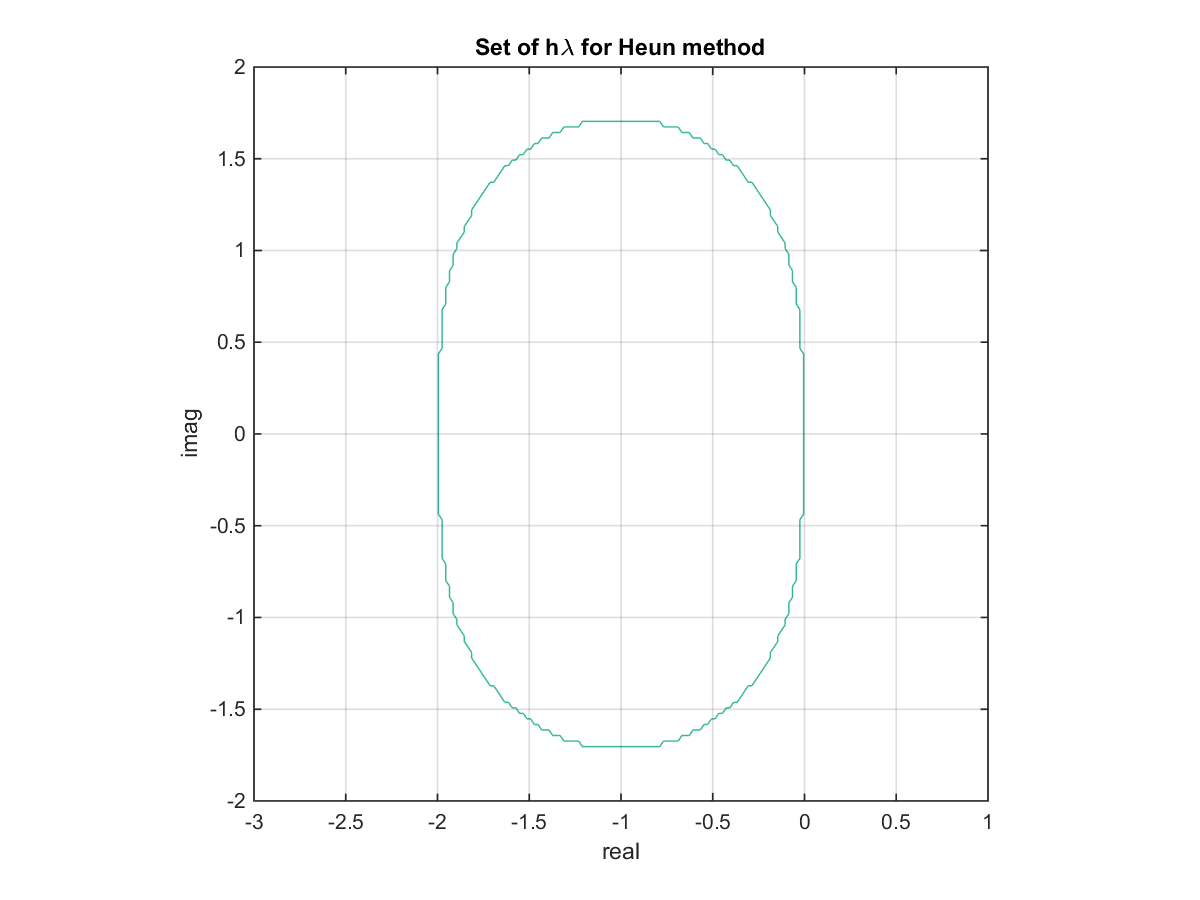
\includegraphics[scale=0.5]{hw6_d1.png}
		\caption{Set of $h\lambda$ for Heun's method}
	\end{figure}\\
	- For Runge-Kutta's method: $|x_k| \rightarrow 0$ as $k \rightarrow \infty \Leftrightarrow \left| 1+ h\lambda + \dfrac{1}{2}h^2\lambda^2 + \dfrac{1}{6}(\lambda h)^3 + \dfrac{1}{24}(\lambda h)^4 \right|<$
	\begin{figure}[htp]
		\centering
		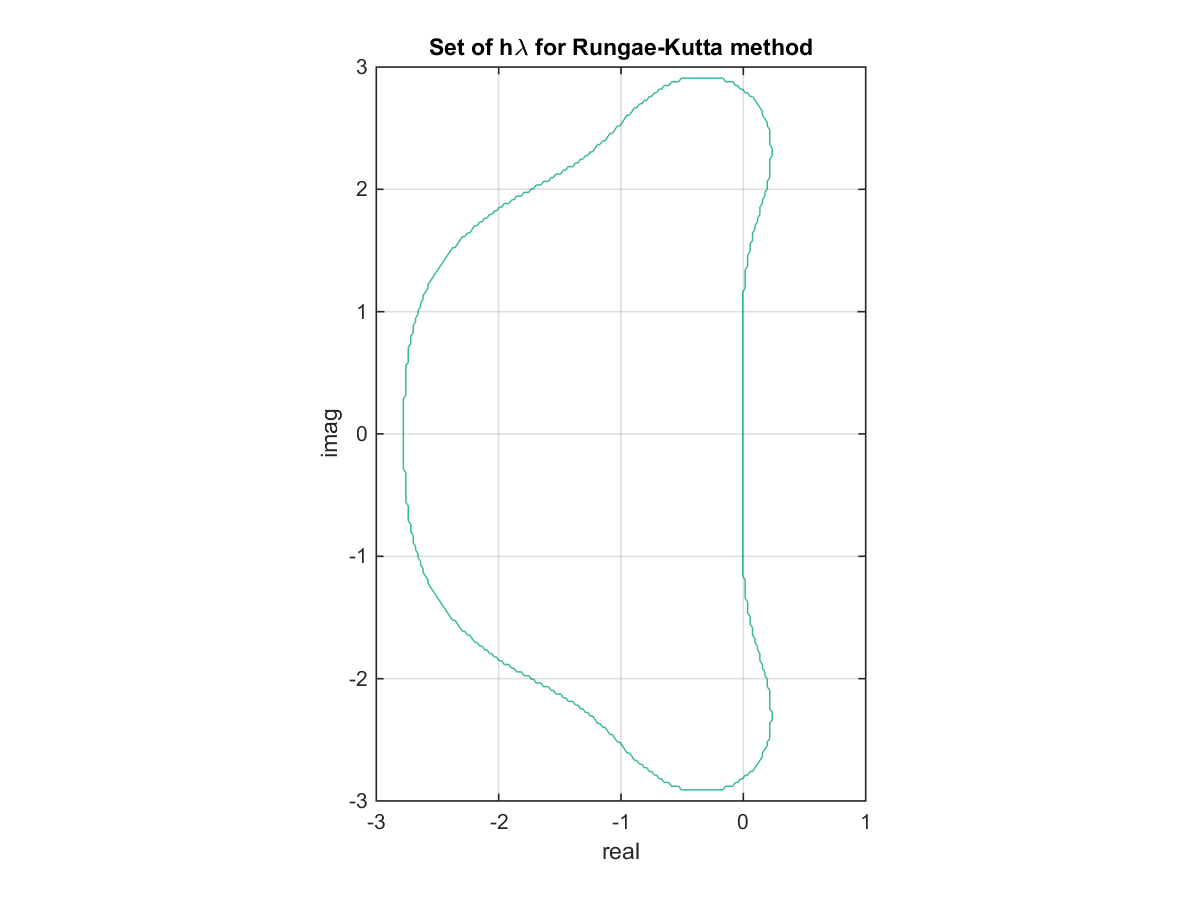
\includegraphics[scale=0.6]{hw6_d2.png}
		\caption{Set of $h\lambda$ for Runge-Kutta's method}
	\end{figure}
	\begin{lstlisting}
	close all; clear all; clc;
	npts = 200;                        % the larger the number, the nicer the plot
	z_real = linspace(-3,1,npts);      % real parts of h*lambda
	z_imag = linspace(-3,3,npts);      % imaginary parts of h*lambda
	[Zr,Zi] = meshgrid(z_real,z_imag); % matrix of real, imag parts
	hLambda = Zr+1i*Zi;                % matrix of complex h*Lambda values
		
	figure; clf;
	contour(z_real,z_imag,abs(1+hLambda + (hLambda.^2)/2 )<1,[1 1]);
	axis equal; grid on;
	axis([min(z_real) max(z_real) min(z_imag) max(z_imag)]);
	
	figure; clf;
	contour(z_real,z_imag,abs(1+hLambda + (hLambda.^2)/2 + (hLambda.^3)/6 + (hLambda.^4)/24 )<1,[1 1]);
	axis equal; grid on;
	axis([min(z_real) max(z_real) min(z_imag) max(z_imag)]);
	
	\end{lstlisting}
		
\end{enumerate}


\label{Problem 2}
\large\textbf{Problem 2.} Consider 2-step linear multistep methods of the form:\\
\hspace*{5cm} $x_{k+2} + Ax_{k+1} + Bx_k = hCf_{k+1}$\\
for the initial value problem $x'(t) = f(t,x(t)), x(t_0) = x_0$, where $A,B$ and $C$ are constants.\\
For 2-step linear multistep we have: 
$$ \sum_{j=0}^{2} \alpha_jx_{k+j} = h\sum_{j=0}^{2}\beta_jf_{k+j}$$
we have: $\alpha_0 = B, \alpha_1 = A, \alpha_2 = 1; \beta_0 = 0, \beta_1 = C, \beta_2 = 0$
\begin{enumerate}
	\label{2a} 
	\item Determine all choices of $A,B$ and $C$ for which this method is consistent.\\
	This method is consistent if:
	\\$\begin{cases} \sum_{j=0}^{2} \alpha_j = 0 \\ \sum_{j=0}^{2} j\alpha_j = \sum_{j=0}^{2} \beta_j \end{cases} \Leftrightarrow \begin{cases} 1 + A + B = 0 \\ 0.B + 1.A + 2.1 = C \end{cases} \Leftrightarrow \begin{cases} A + B = -1 \\ A = C-2 \end{cases}$\\
		
	\label{2b}	
	\item Determine a choice $A,B$ and $C$ that gives $O(h^2)$ truncation error.\\
	The truncation error is $0(h^2)$ if for $ l = 1,2$:\\
	$\begin{cases} \sum_{j=0}^{2} \alpha_j = 0 \\ \sum_{j=0}^{2} \dfrac{j^l}{l!}\alpha_j = \sum_{j=0}^{2} \dfrac{j^{l-1}}{(l-1)!}\beta_j \end{cases} \Leftrightarrow \begin{cases} \sum_{j=0}^{2} \alpha_j = 0 \\ \sum_{j=0}^{2} j\alpha_j = \sum_{j=0}^{2} \beta_j \\ \sum_{j=0}^{2} \dfrac{j^2}{2}\alpha_j = \sum_{j=0}^{2} j\beta_j \end{cases} \Leftrightarrow \begin{cases} 1 + A + B = 0 \\ 0.B + 1.A + 2.1 = C \\ \dfrac{0}{2}B + \dfrac{1}{2}A + \dfrac{2^2}{2}.1 = C \end{cases}$\\
	\hspace*{2cm} $ \Leftrightarrow \begin{cases} A + B = -1 \\ A = C-2 \\ A = 2C -4 \end{cases}  \Leftrightarrow \begin{cases} A=0 \\ B = -1 \\ C =2 \end{cases} $\\
			
	\label{2c}
	\item Access the zero-stability of the method found in part (b).\\
	We have characteristic polynomial of the LMM is: 
	$$p(\gamma) = \sum_{j=0}^{2}\alpha_j\gamma^j = -1 + \gamma^2 = (\gamma - 1)(\gamma +1)$$
	Characteristic polynomial have 2 roots: $\gamma = 1$ and $\gamma = -1 \Rightarrow$ zero-stable.
		
	\label{2d}
	\item What does your answer to part (c) imply about the behavior of the linear multistep method as $h \rightarrow 0$ for such value $A,B$ and $C$?\\
	we have the exact solution for: $x'(t) = \lambda x(t)$ is $x(t) = e^{\lambda t}x(0)$ with $\lambda = \gamma + \delta i$\\
	based on part (c) result: $\gamma = \pm 1$ and $\delta = 0$ so:\\
	+ for $\gamma = 1$: $x(t) = e^tx(0) \Rightarrow$ for $t \rightarrow \infty: x(t) \rightarrow \infty$\\
	+ for $\gamma = -1$: $x(t) = e^{-t}x(0) \Rightarrow$ for $t \rightarrow \infty: x(t) \rightarrow 0$
	
	\label{2e} 
	\item For the method found in part (b), calculate those values of $\lambda h$ for which $x_k \rightarrow 0$ as $k \rightarrow \infty$ when applied to the differential equation $x' = \lambda x$.\\
	As $A = 0, B = -1, C= 2$ and $x' = \lambda x$, we have: $x_{k+2} - x_k = 2h\lambda x_{k+1}$\\
	For $x_k = \gamma^k$, the stability polynomial is: $p(\gamma) - h\lambda\sigma(\gamma) = 0$
	$$p(\gamma) - h\lambda\sigma(\gamma) = \sum_{j=0}^{2}\alpha_j\gamma^j - h\lambda\sum_{j=0}^{2}\beta_j\gamma^j = -1 + \gamma^2 - h\lambda(2\gamma) = 0$$
	$\Delta = 4h^2\lambda^2 + 4 \Rightarrow \gamma = \dfrac{2h\lambda \pm \sqrt{4h^2\lambda^2 + 4}}{2} = h\lambda \pm \sqrt{h^2\lambda^2 +1}$\\
	Stability condition: $|\gamma| = |h\lambda \pm \sqrt{h^2\lambda^2 +1}| <1$\\
	With two different values of $\gamma$ we have two set of $h\lambda$ respectively: 
	\begin{figure}[htp]
		\centering
		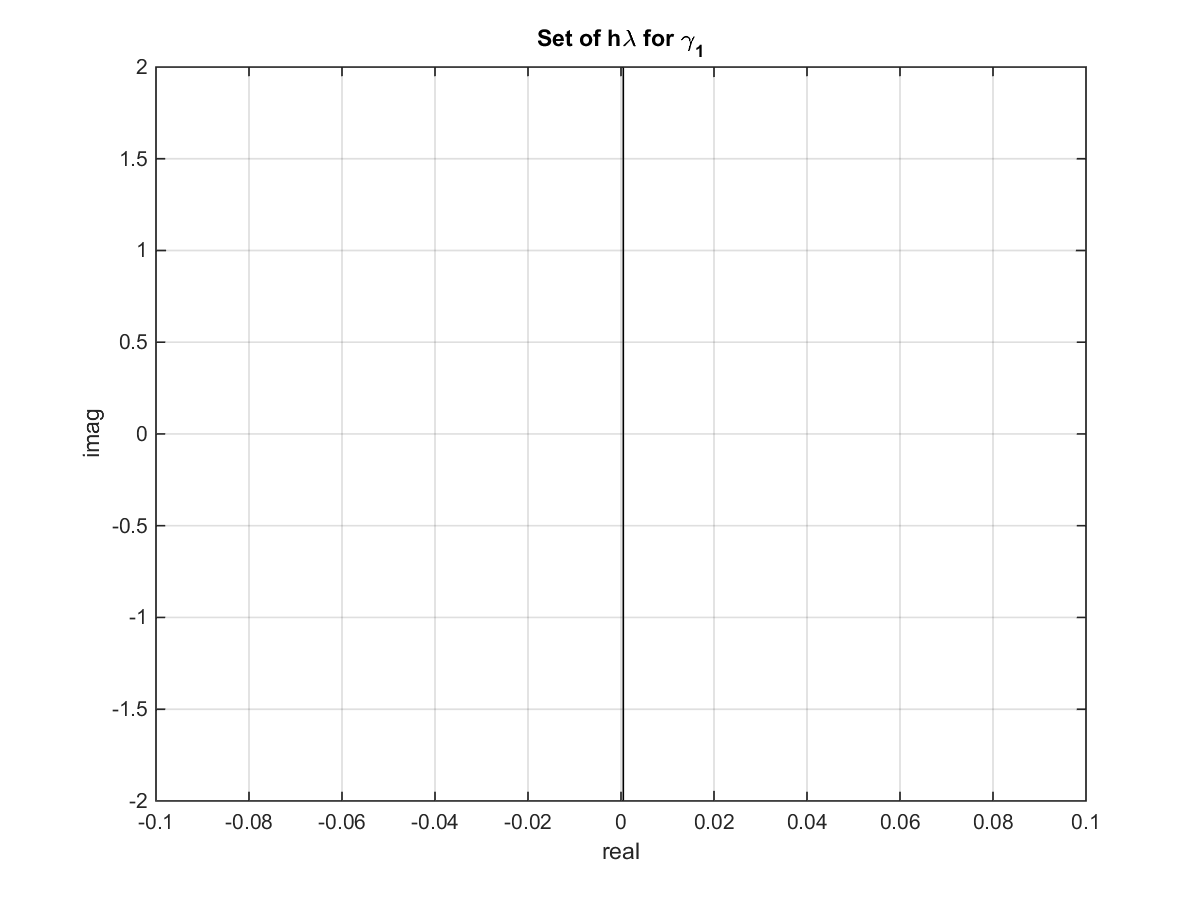
\includegraphics[scale=0.5]{hw6_2e1.png}
		\caption{Set of $h\lambda$ for $\gamma_1 = h\lambda - \sqrt{h^2\lambda^2 +1}$}
	\end{figure}\\
	\begin{figure}[htp]
		\centering
		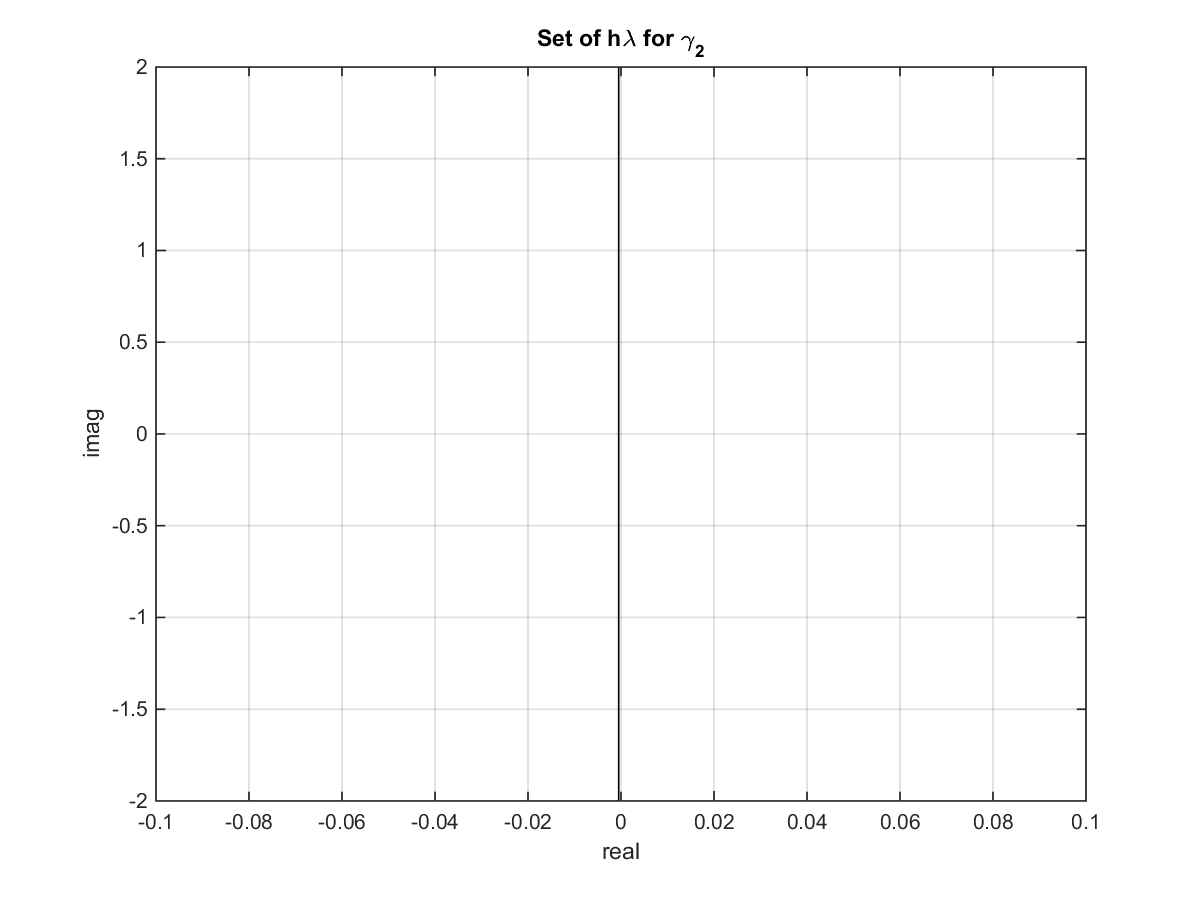
\includegraphics[scale=0.5]{hw6_2e2.png}
		\caption{Set of $h\lambda$ for $\gamma_2 = h\lambda + \sqrt{h^2\lambda^2 +1}$}
	\end{figure}
	\begin{lstlisting}
npts = 200;                        
z_real = linspace(-0.1,0.1,npts);   
z_imag = linspace(-2,2,npts);     
[Zr,Zi] = meshgrid(z_real,z_imag); 
hLambda = Zr+1i*Zi;                
figure; clf; 
contour(z_real,z_imag,abs(hLambda - sqrt(hLambda.^2 +1) )<1,[1 1],'k');
grid on; xlabel('real'); ylabel('imag');
title('Set of h\lambda for \gamma_1'); print('hw6_2e1','-dpng');
figure; clf; 
contour(z_real,z_imag,abs(hLambda + sqrt(hLambda.^2 +1) )<1,[1 1],'k');
grid on; xlabel('real'); ylabel('imag');
axis([min(z_real) max(z_real) min(z_imag) max(z_imag)])
title('Set of h\lambda for \gamma_2'); print('hw6_2e2','-dpng');
	\end{lstlisting}
	%Set of $h\lambda$ in both cases are really small.
\end{enumerate}

\label{Problem 3}
\large\textbf{Problem 3.} \textit{Convection-diffusion equation} play an important role in fluid dynamics. In one dimension, the simplest such equation takes the form: $-\varepsilon u''(x) + u'(x) = 0; u(0) = a, u(1) = b$\\
(The second derivative term, $\Lambda u$ in higher dimensions, gives diffusion; the first derivative term, $\textbf{w}^Tu$ in higher dimensions, gives convection in the direction of the 'wind', \textbf{w}).
Note that this convection-diffusion equation is a \textit{boundary value problem}, rather than an initial value problem. As stated, it is easy enough to solve by hand, but it will be useful to develop a numerical method that we could also apply to more difficult problems. The \textit{shooting method} is one option:\\
$\bullet$ Write this second-order ODE as a system of two first-order ODEs: $\begin{cases} u_1'(x) = u_2(x) \\ u_2'(x) = \varepsilon^{-1}u_2(x) \end{cases}$\\
$\bullet$ Guess some value for $u'(0)$.
$\bullet$ Integrate this system (e.g., using a Runge-Kutta method) for $x \in [0,1]$ with the initial values $u_1(0) = u(0) = a$ (given by the problem) and $u_2 = u'(0)$ (guessed).\\
$\bullet$ Unless you are lucky, the solution you obtain will not match the boundary condition $u(1) = b$, because the guessed value for $u'(0)$ is not correct. One can use a nonlinear root finding algorithm (e.g., bisection, \textit{regular falsi} the secant method, or Newton's method to adjust the guess $u'(0)$ until the integrated value at $x = 1$ agrees with the desired $u(1) = b$. That is, one seeks a zero of the objective function: $f(\xi) = b-(u(1)$ computed with $u'(0) = \xi)$\\
The following figure shows a schematic view of the shooting method (for a different differential equation). The solid line is the solution to the ODE with the correct value $u(0) = a$, but the incorrect $u'(0)$. Since this initial slope is incorrect, the corresponding value for $u(1)$ is also wrong. The dashed line shows the true solution, which satisfies $u(1) = b$. The challenge is to adjust the guessed value for $u'(0)$ so that the computed $u(1)$ satisfies the boundary condition $u(1) = b$.\\
Your task is to solve the convection-diffusion equation.
\begin{enumerate}
	\label{3a}
	\item Implement the shooting method to solve the above convection-diffusion boundary value problem with $\varepsilon = 1/10, u(0) = 0$, and $u(1) = 1$. Please use \texttt{MATLAB}'s built-in ODE integrator, \texttt{ode45}; you may use any root-finding algorithm you like, but please implement it yourself or use the codes on the class website. If you use the bisection or \textit{regula falsi} algorithm, use $u'(0) = 0$ and $u'(0) = 1$ to obtain your initial bracket. If you use the secant method of Newton's method, try $u'(0) = 0$ as an initial guess.\\
	Please present your code, a pilot of $u(x)$ for $ x \in [0,1]$, and the value of $u'(0)$ that gives $u(1) = 1$.\\
	We have: $u'(x) = u_1(x), u''(x) = \varepsilon^{-1}u_2(x) = 10u_2(x)$. So:\\
	\hspace*{2cm} $\begin{bmatrix} u_1'(x) \\ u_2'(x) \end{bmatrix} = \begin{bmatrix} 0&1\\1&10 \end{bmatrix} \begin{bmatrix} u_1(x)\\u_2(x) \end{bmatrix} \Leftrightarrow u'(x) = \begin{bmatrix} 0&1\\1&10 \end{bmatrix} u(x)$\\
	Apply \texttt{ode45} function in \texttt{MATLAB}:
	\begin{lstlisting}
	close all; clear all;
	[t,x] = ode45(@(t,x) [0 1;0 10]*x, [0 1], [0;0.00045395]);
	figure; plot(t,x(:,1),'r'); grid on;
	xlabel('x'); ylabel('u(x)');
	title('Approximation for u(x) utilizing ode45, \epsilon = 10');
	print('hw6_3a','-dpng');
	\end{lstlisting}
	\begin{figure}[htp]
		\centering
		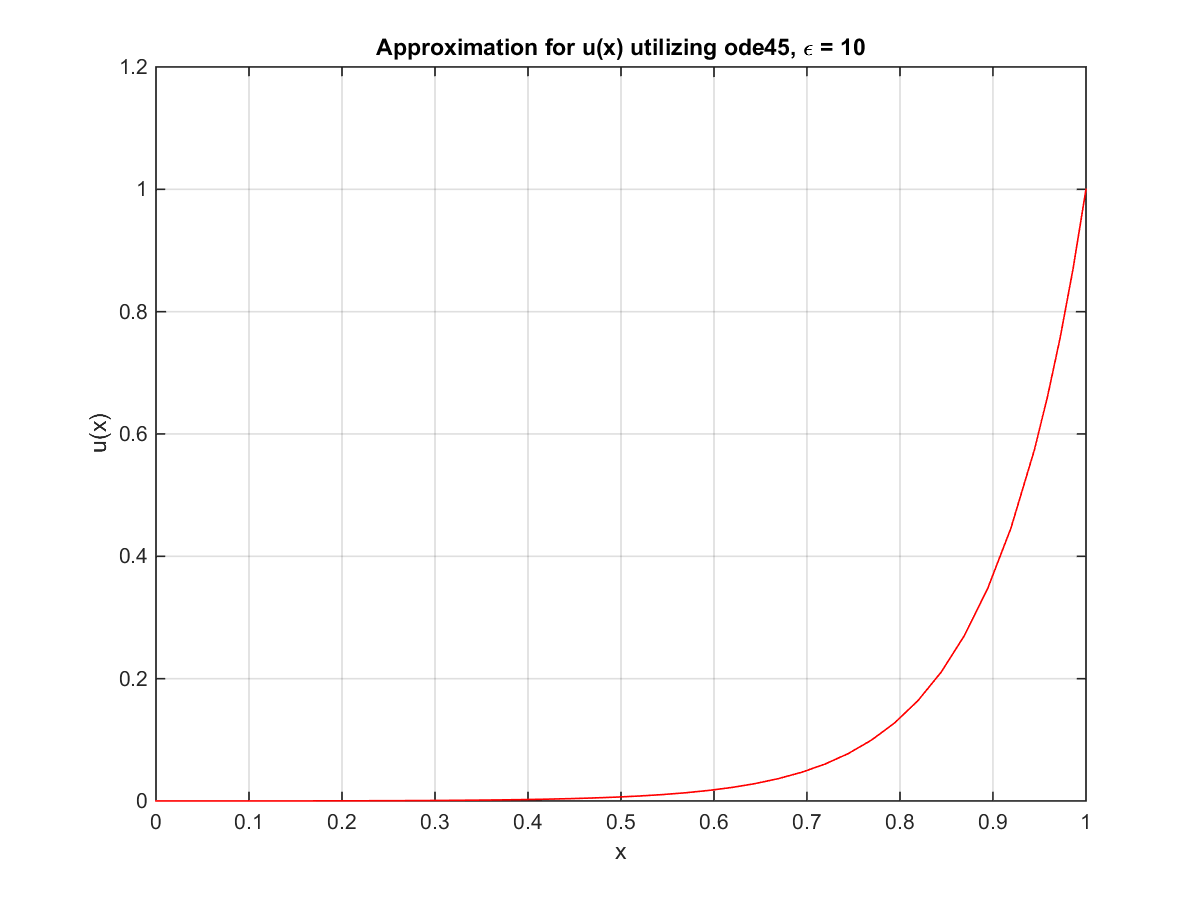
\includegraphics[scale=0.5]{hw6_3a.png}
		\caption{Approximation of $u(x)$ for convection-diffusion problem with $\varepsilon = 10$}
	\end{figure}
	
	\label{3b}
	\item Repeat the same experiment for $\varepsilon = 1/50$ The exact solution demonstrates a \textit{boundary layer} near $x =1$.
	\begin{lstlisting}
	close all; clear all;
	[t,x] = ode45(@(t,x) [0 1;0 50]*x, [0 1], [0;0.50395e-19]);
	figure; plot(t,x(:,1),'r'); grid on;
	xlabel('x'); ylabel('u(x)');
	title('Approximation for u(x) utilizing ode45, \epsilon = 50');
	print('hw6_3b','-dpng');
	\end{lstlisting}
	\begin{figure}[htp]
		\centering
		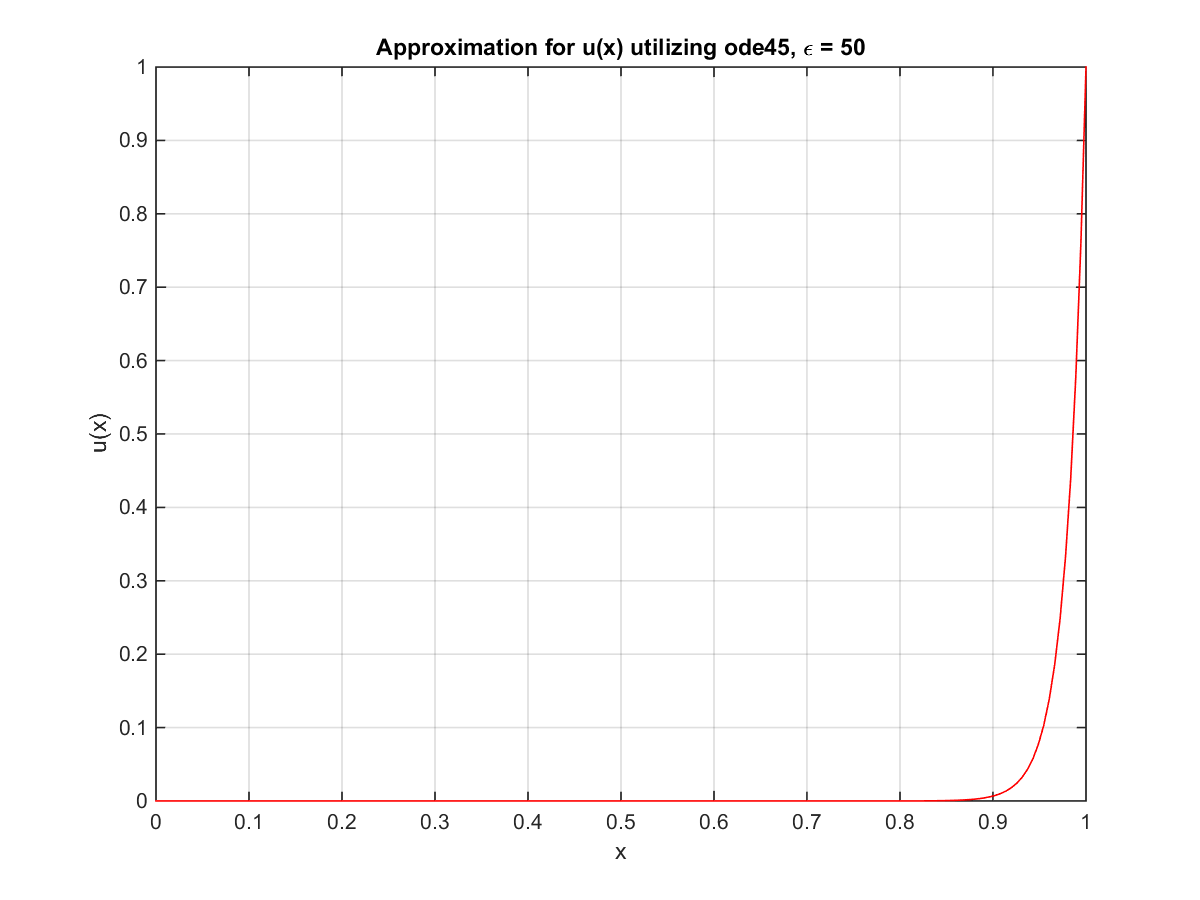
\includegraphics[scale=0.5]{hw6_3b.png}
		\caption{Approximation of $u(x)$ for convection-diffusion problem with $\varepsilon = 10$}
	\end{figure}
	
	\label{3c}
	\item Derive the exact solution for this convection-diffusion problem. In particular, what are the exact values for $u'(0)$ in part (a) and (b)? How do these values of $u'(0)$ compare to those you computed in (a) and (b)?\\
	Assume one possible solution for $u(x)$ is: $u(x) = e^{\lambda x}$, so: $u'(x) = \lambda e^{\lambda x}, u''(x) = \lambda^2e^{\lambda x}$\\
	Replace into convection-diffusion problem we have:\\
	\hspace*{2cm} $-\varepsilon\lambda^2e^{\lambda x} + \lambda e^{\lambda x} = 0 \Leftrightarrow \lambda(1 - \varepsilon\lambda)e^{\lambda x} = 0 \Leftrightarrow \begin{cases} \lambda_1 = 0 \\ \lambda_2 = \dfrac{1}{\varepsilon} \end{cases}$\\
	We have the general solution: $u(x) = c_1e^{\lambda_1x} + c_2e^{\lambda_2x} = c_1e^{0.x} + c_2e^{\frac{1}{\varepsilon}x} = c_1 + c_2e^{x/\varepsilon}$\\
	For initial condition: $u(0) = 0$ and $u(1) = 1$: $\begin{cases} u(0) = c_1 + c_2 = 0 \\ u(1) = c_1 + c_2e^{1/\varepsilon} = 1 \end{cases} \Leftrightarrow \begin{cases} c_1 = -\dfrac{1}{e^{1/\varepsilon}-1} \\ c_2 = \dfrac{1}{e^{1/\varepsilon}-1} \end{cases} $\\
	Exact solution for convection-diffusion problem: $u(x) = -\dfrac{1}{e^{1/\varepsilon}-1} + \dfrac{1}{e^{1/\varepsilon}-1}e^{x/\varepsilon}$\\
	$\Rightarrow u'(x) = \dfrac{1}{\varepsilon(e^{1/\varepsilon}-1)}e^{x/\varepsilon}$\\
	For part (a): $\varepsilon = 1/10 \Rightarrow u(x) = - \dfrac{1}{e^{10}-1} + \dfrac{1}{e^{10}-1}e^{10x}$\\
	\hspace*{2.5cm} $u'(x) = \dfrac{1}{10(e^{10}-1)}e^{10x} \hspace{0.5cm} \rightarrow \hspace{0.5cm} u'(0) = \dfrac{1}{10(e^{10}-1)}e^0 = 4.5402 \times 10^{-6} $ \\
	For part (a): $\varepsilon = 1/50 \Rightarrow u(x) = - \dfrac{1}{e^{50}-1} + \dfrac{1}{e^{50}-1}e^{50x}$\\
	\hspace*{2.5cm} $u'(x) = \dfrac{1}{50(e^{50}-1)}e^{50x} \hspace{0.5cm} \rightarrow \hspace{0.5cm} u'(0) = \dfrac{1}{50(e^{50}-1)}e^0 = 3.8575 \times 10^{-24} $ \\
	The guessed value for $u'(0)$ in both part (a) and (b) are bigger than the real values:\\
	\hspace*{1cm} $ 0.00045395 > 4.5402 \times 10^{-6} $ \hspace{0.3cm} and \hspace{0.3cm} $ 0.50395e-19 >  3.8575 \times 10^{-24} $ \\
\end{enumerate}

\label{Problem 4}
\large\textbf{Problem 4.} \textbf{Method of Lines}. Many physical models give rise to time-dependent partial differential equations. General techniques to solve such problems are beyond the scope of this course. However, many such problems can be attacked using standard OED integrators via a technique known as the \textit{method of lines}. In this problem, you will solve the \textit{first-order wave equation}: $u_t(t,x) = u_x(t,x)$\\
Here $u(t,x)$ is a scalar function of two real variables, $u_t$ denotes the time derivative, and $u_x$ denotes the space derivative. The problem is posed on the temporal domain $t \geq 0$ and spatial domain $x \in (-\infty, \infty)$. The initial data will be: $u(0,x) = \sin(2\pi x)$.\\
which gives the exact solution: $u(t,x) = \sin(2\pi(x+t))$\\
The method of the lines approximates the solution to a partial differential equation by first discretizing the domain on the $x$-direction into points $x_j = j\Delta x$, where $\Delta x = 1/n$ for some fixed $n$. Since the initial data is periodic, we only need to discretize from $x_1 = \Delta x$ through $x_n = n\Delta x = 1$, and then assign $x_0 = x_n$ by periodicity.\\
Now approximate the spatial $(x)$ derivative by the simple finite difference approximation:\\
\hspace*{4cm} $u_x(t,x_j) \approx \dfrac{u(t,x_{j+1}) - u(t,x_j)}{\Delta x}; $ \\
we have previously observed that this approximation incurs an $0(\Delta x)$ error. The method of lines approximates the partial differential equation $u_t = u_x$ with an \textit{ordinary differential equation} by replacing $u_x$ with the finite differential approximation, giving:\\
\hspace*{4cm} $u_t(t,x_j) = \dfrac{u(t,x_{j+1}) - u(t,x_j)}{\Delta x}$\\
Exploiting periodicity (which implies that $u(t,x_n) = u(t,x_0)$), this reduces the partial differential equation to a system of $n$ ordinary differential equations. Using the notation.\\
\hspace*{5cm} $\textbf{u}(t) = \begin{bmatrix} u(t,x_1)\\ u(t,x_2) \\ ... \\ u(t,x_n) \end{bmatrix} \in \mathbb{R}^n$ \\
this system of differential equation can be written as: $\textbf{u}_t(t) = \textbf{Au}(t)$
\begin{enumerate}
	\label{4a}
	\item What is the matrix $\textbf{A} \in \mathbb{R}^{n\times n}$ ? (Be careful not to neglect the entry that arises because of periodicity)\\
	We have: $x_{n+1} = (n+1)\Delta x = 1 + \Delta x$\\
	As definition of $u(t,x)$:\\ $u(t,x_{n+1}) = \sin(2\pi(t+x_{n+1})) = sin(2\pi(t+ 1 + \Delta x)) = \sin(t+\Delta x) = \sin(t+x_1) = u(t,x_1)$ \\
	So: $u_t(t,x_n) = \dfrac{u(t,x_{n+1}) - u(t,x_n)}{\Delta x} = \dfrac{u(t,x_1) - u(t,x_n)}{\Delta x}$\\
	and: $u_t(t,x_j) = \dfrac{u(t,x_{j+1}) - u(t,x_j)}{\Delta x}$ \hspace*{1cm} for $j = 1, ..., n-1$\\ 
	We come up with:\\
	\hspace*{2cm} $\textbf{u}_t(t) = \textbf{Au}(t) = \dfrac{1}{\Delta x}\begin{bmatrix} -1&1&0&0 & ...&... &0 \\ 0&-1&1&0& ...&... &0 \\ &... & & ... && ... \\0&0&0&0&... &-1&1 \\ 1& 0&0&0 & ...&... &-1 \end{bmatrix} \begin{bmatrix} u(t,x_1)\\ u(t,x_2) \\ ... \\ u(t,x_n) \end{bmatrix} $\\
	So we have $\textbf{A} \in \mathbb{R}^{n\times n}$: $\textbf{A} = \begin{bmatrix} -\dfrac{1}{\Delta x}&\dfrac{1}{\Delta x}&0&0 & ...&... &0 \\ 0&-\dfrac{1}{\Delta x}&\dfrac{1}{\Delta x}&0& ...&... &0 \\ &... & & ... && ... \\0&0&0&0&... &-\dfrac{1}{\Delta x}&\dfrac{1}{\Delta x} \\ \dfrac{1}{\Delta x}& 0&0&0 & ...&... &-\dfrac{1}{\Delta x}\end{bmatrix}$ \\
	
	\label{4b}	
	\item Verify (by proving analytically, or by simply computing a numerical example for $n =7$, whichever you prefer) that \textbf{A} has the $n$ eigenvalues and associated eigenvectors.\\
	\hspace*{0.5cm} $\lambda_j = (e^{i\theta_j} - 1)/\Delta x$, \hspace{0.3cm} $\textbf{v}_j = (e^{i\theta_j}, e^{2i\theta_j}, ..., e^{ni\theta_j})^T$ \hspace{0.3cm} for $\theta_j = 2\pi j/n$ for $j = 1, ..., n$
	
	For n = 7 we will have the eigenvalues of matrix \textbf{A} is defined by:
	\begin{align*}\det[\lambda\mathrm{I} - \textbf{A}] &= \det \begin{bmatrix} \lambda +\dfrac{1}{\Delta x}&-\dfrac{1}{\Delta x}&0&0 & 0&0 &0 \\ 0&\lambda+\dfrac{1}{\Delta x}&-\dfrac{1}{\Delta x}&0& 0&0 &0 \\ 0&0& \lambda +\dfrac{1}{\Delta x}&-\dfrac{1}{\Delta x} &0&0&0 \\ 0&0&0& \lambda +\dfrac{1}{\Delta x}&-\dfrac{1}{\Delta x} &0&0 \\ 0&0&0&&0 \lambda +\dfrac{1}{\Delta x}&-\dfrac{1}{\Delta x} &0 \\0&0&0&0&0&\lambda+\dfrac{1}{\Delta x}&-\dfrac{1}{\Delta x} \\ -\dfrac{1}{\Delta x}& 0&0&0 &0 &0 &\lambda +\dfrac{1}{\Delta x}\end{bmatrix} \\
	&= \left(\lambda+\dfrac{1}{\Delta x}\right)^7 + \left(\dfrac{-1}{\Delta x} \right)^7 \end{align*} 
	with $\lambda = \dfrac{e^{i\theta_j}-1}{\Delta x}$: $ \det[\lambda\mathrm{I} - \textbf{A}] = \left(\dfrac{e^{i\theta_j}-1}{\Delta x}+\dfrac{1}{\Delta x}\right)^7 + \left(\dfrac{-1}{\Delta x} \right)^7 = \dfrac{1}{(\Delta x)^7}(e^{7i\theta_j} - 1)$\\
	$e^{7i\theta_j} + 1 = \cos\left(7*\dfrac{2\pi j}{7}\right) + i\sin\left(7*\dfrac{2\pi j}{7}\right) - 1 = \cos(2\pi j) + i\sin(2\pi j) 1 1 = 1 + i*0 - 1 = 0$\\
	$\Rightarrow \det[\lambda\mathrm{I} - \textbf{A}] = 0$ for $n = 7$ and $j = 1,2,...,7$\\
	$\Rightarrow \lambda = \dfrac{e^{i\theta_j}-1}{\Delta x}$ are eigenvalues of \textbf{A} (with $j = 1,2,...,7)$\\
	
	For eigenvalues and eigenvectors of matrix \textbf{A} we will have: $\lambda_jv_j = \textbf{A}v_j $: \\
	$\lambda_jv_j = \dfrac{e^{i\theta_j}-1}{\Delta x}\begin{bmatrix} e^{i\theta_j} \\ e^{2i\theta_j} \\ e^{3i\theta_j} \\ e^{4i\theta_j} \\ e^{5i\theta_j} \\ e^{6i\theta_j} \\ e^{7i\theta_j} \end{bmatrix} = \dfrac{1}{\Delta x} \begin{bmatrix} e^{i\theta_j}(e^{i\theta_j}-1) \\ e^{2i\theta_j}(e^{i\theta_j}-1) \\ e^{3i\theta_j}(e^{i\theta_j}-1) \\ e^{4i\theta_j}(e^{i\theta_j}-1) \\ e^{5i\theta_j}(e^{i\theta_j}-1) \\ e^{6i\theta_j}(e^{i\theta_j}-1) \\ e^{7i\theta_j}(e^{i\theta_j}-1) \end{bmatrix} = \dfrac{1}{\Delta x} \begin{bmatrix} - e^{i\theta_j} +  e^{2i\theta_j}  \\ - e^{2i\theta_j} + e^{3i\theta_j} \\ - e^{3i\theta_j} + e^{4i\theta_j} \\ - e^{4i\theta_j}+ e^{5i\theta_j} \\ - e^{5i\theta_j} + e^{6i\theta_j} \\ - e^{6i\theta_j} + e^{7i\theta_j} \\ - e^{7i\theta_j} + e^{8i\theta_j}\end{bmatrix}  $\\
	
	$\textbf{Av}_j = \dfrac{1}{\Delta x}\begin{bmatrix} -1&1&0&0 & 0&0 &0 \\ 0&-1&1&0& 0&0 &0 \\ 0&0& -1&1&0&0&0 \\ 0&0&0& -1&1&0&0 \\ 0&0&0&&0 -1&1&0 \\0&0&0&0&0&-1&1 \\ -1& 0&0&0 &0 &0 &-1\end{bmatrix} \begin{bmatrix} e^{i\theta_j} \\ e^{2i\theta_j} \\ e^{3i\theta_j} \\ e^{4i\theta_j} \\ e^{5i\theta_j} \\ e^{6i\theta_j} \\ e^{7i\theta_j} \end{bmatrix} = \dfrac{1}{\Delta x} \begin{bmatrix} - e^{i\theta_j} +  e^{2i\theta_j}  \\ - e^{2i\theta_j} + e^{3i\theta_j} \\ - e^{3i\theta_j} + e^{4i\theta_j} \\ - e^{4i\theta_j}+ e^{5i\theta_j} \\ - e^{5i\theta_j} + e^{6i\theta_j} \\ - e^{6i\theta_j} + e^{7i\theta_j} \\ - e^{7i\theta_j} + e^{i\theta_j}\end{bmatrix}  $\\
	We have: $e^{8i\theta_j} = \cos(8\theta_j) + i\sin(8\theta_j) = \cos\left(8*\dfrac{2\pi j}{7}\right) +i\sin \left(8*\dfrac{2\pi j}{7}\right)\\ \hspace*{6.65cm} = \cos\left(2\pi j + \dfrac{2\pi j}{7}\right) + i\sin\left(2\pi j + \dfrac{2\pi j}{7}\right)\\ \hspace*{6.65cm} = \cos\left(\dfrac{2\pi j}{7}\right) + i\sin\cos\left(\dfrac{2\pi j}{7}\right) = \hspace*{0.5cm} e^{i\theta_j}$ \hspace{0.2cm} (*)\\
	$\Rightarrow - e^{7i\theta_j} + e^{8i\theta_j} =  - e^{7i\theta_j} + e^{i\theta_j} \Leftrightarrow \lambda_jv_j = \textbf{Av}_j$ \hspace{1cm} for $j = 1,2, ...,7$\\
	(*) is right for $n < 8$ or maximum value of $n$ is 7 or \textbf{A} has $n=7$ eigenpairs: $\lambda_j$ and $v_j$.\\
	
	Finally, the method of lines solves $\textbf{u}_t = \textbf{Au}$ using an ODE integrator. For simplicity, use the forward Euler method: \hspace{2cm} $\textbf{u}_{k+1} = \textbf{u}_k + \Delta t\textbf{Au}_k$	
	\label{4c}
	\item Consider the eigenvalues from part (b), together with the theory of absolute stability for the forward Euler method, to determine a sharp condition on $\Delta t$ that ensures there are no exponentially growing solutions for a fixed value of $\Delta x$. \\%(You have just derived the famous \textit{CFL condition}, first noted in a seminal 1928 paper by Richard Courant, Kurt Otto Friedrichs, and Hans Lewy).\\
	\hspace*{2cm} $\textbf{u}_{k+1} = \textbf{u}_k + \Delta t\textbf{Au}_k \Leftrightarrow \textbf{u}_{k+1} = (I + \Delta t\textbf{A})\textbf{u}_k  \Rightarrow \gamma = I + \Delta t\textbf{A} $\\	
	As above result with $\lambda_j, v_j$ are eigenpairs of \textbf{A}: $\textbf{A} = V\Lambda V^{-1}$ 	\\
	$ \textbf{A} = \begin{bmatrix} e^{i\theta_1} & e^{i\theta_2} & ... & e^{i\theta_n} \\ e^{2i\theta_1} & e^{2i\theta_2} & ... & e^{2i\theta_n} \\ ... & ... & ... & ... \\ e^{ni\theta_1} & e^{ni\theta_2} & ... & e^{ni\theta_n} \end{bmatrix} \begin{bmatrix} \dfrac{e^{i\theta_1}-1}{\Delta x} & 0 & ... & 0 \\ 0& \dfrac{e^{i\theta_2}-1}{\Delta x}& ... &0 \\ ... &...&...&... \\ 0&0&...&\dfrac{e^{i\theta_n}-1}{\Delta x} \end{bmatrix} \begin{bmatrix} e^{i\theta_1} & e^{i\theta_2} & ... & e^{i\theta_n} \\ e^{2i\theta_1} & e^{2i\theta_2} & ... & e^{2i\theta_n} \\ ... & ... & ... & ... \\ e^{ni\theta_1} & e^{ni\theta_2} & ... & e^{ni\theta_n} \end{bmatrix}^{-1}$\\
	Iterating from initial condition: $x_1 = (I + \Delta t\textbf{A})x_0$\\
	\hspace*{5.7cm} $x_2 = (I + \Delta t\textbf{A})x_1 = (I + \Delta t\textbf{A})^2x_0$ ...\\
	\hspace*{2.5cm} or in general: \hspace{0.5cm}  $x_k = (I + \Delta t\textbf{A})^kx_0$\\
	$\Rightarrow$ the stable condition is: $|\gamma| = \left| I + \Delta t\textbf{A}\right| < 1$ \hspace{5cm} (***)\\
	The above condition will be satisfied if all the eigenvalues of $[\textbf{I} + \Delta t\textbf{A}]$ are less than 1.\\
	Due to \textit{spectral mapping theorem}: if $(\lambda_j,v_j)$ is an eigenpairs of \textbf{A} $\rightarrow (1 + \Delta t\lambda_j,\textbf{v}_j)$ is an eigenpair of $[\textbf{I} + \Delta t\textbf{A}]$, then:\\
	\hspace*{3cm} $[\textbf{I} + \Delta t\textbf{A}]\textbf{v}_j = \textbf{v}_j + \Delta t\textbf{Av}_j = (1 +\Delta t\lambda_j)\textbf{v}_j$\\
	$\Rightarrow x_k$ will decay to 0 if $|1+\Delta t\lambda_j| < 1$ for all $\lambda_j$\\
	This condition is equivalent with: $|1+\Delta t\lambda_j| < 1 \Leftrightarrow -2 < \Delta t\lambda_j < 0$\\
	We have: $\Delta t\lambda_j = \Delta t \dfrac{e^{i\theta_j}-1}{\Delta x} = \dfrac{\Delta t}{\Delta x}(\cos\theta_j + i\sin\theta_j -1)$\\
	So: $|1+\Delta t\lambda_j| < 1 \Leftrightarrow -2 < \dfrac{\Delta t}{\Delta x}(\cos\theta_j + i\sin\theta_j -1) < 0$ \hspace{5cm} (****)\\
	Besides, the set of $(\cos\theta_j + i\sin\theta_j -1)$ is a circle in complex space with center at $-1$ and radius is $1$, mean that $-2 < (\cos\theta_j + i\sin\theta_j -1) < 0$\\
	In order to get (****) is true will all $j$: $\dfrac{\Delta t}{\Delta x} < 1$\\
	
	\label{4d}
	\item Implement your algorithm in \texttt{MATLAB} to confirm that your answer to (c) is correct. In particular, take $\Delta x = 1/50, (n = 50)$ and give solutions when $\Delta t$ is (1) twice the maximum and (2) equal to the maximum allowed by the stability requirement from (c).\\
	You may show this data in several ways: You can plot the solution at time $t =2$ in two dimensions ($u(2,x)$ versus $x$), or in three dimensions for $t \in [0,2]$. For the later, the following \texttt{MATLAB} commands may prove useful: \texttt{surf, mesh, waterfall, pcolor, shading interp}.\\
	The solution for this equation is: $x_k = (\textbf{I} + \Delta t\textbf{A})^kx_0$\\
	Due to above result, the maximum value of $\Delta t$ is $\Delta t = \Delta x$, so:\\
	- When $\Delta t$ is twice the maximum: $\Delta t = 2\Delta x = 2*1/50 = 1/25$\\
	For $t = 2$, the step needed is $k = t/\Delta t = 2/(1/25) = 50$\\
	\begin{figure}[htp]
		\centering
		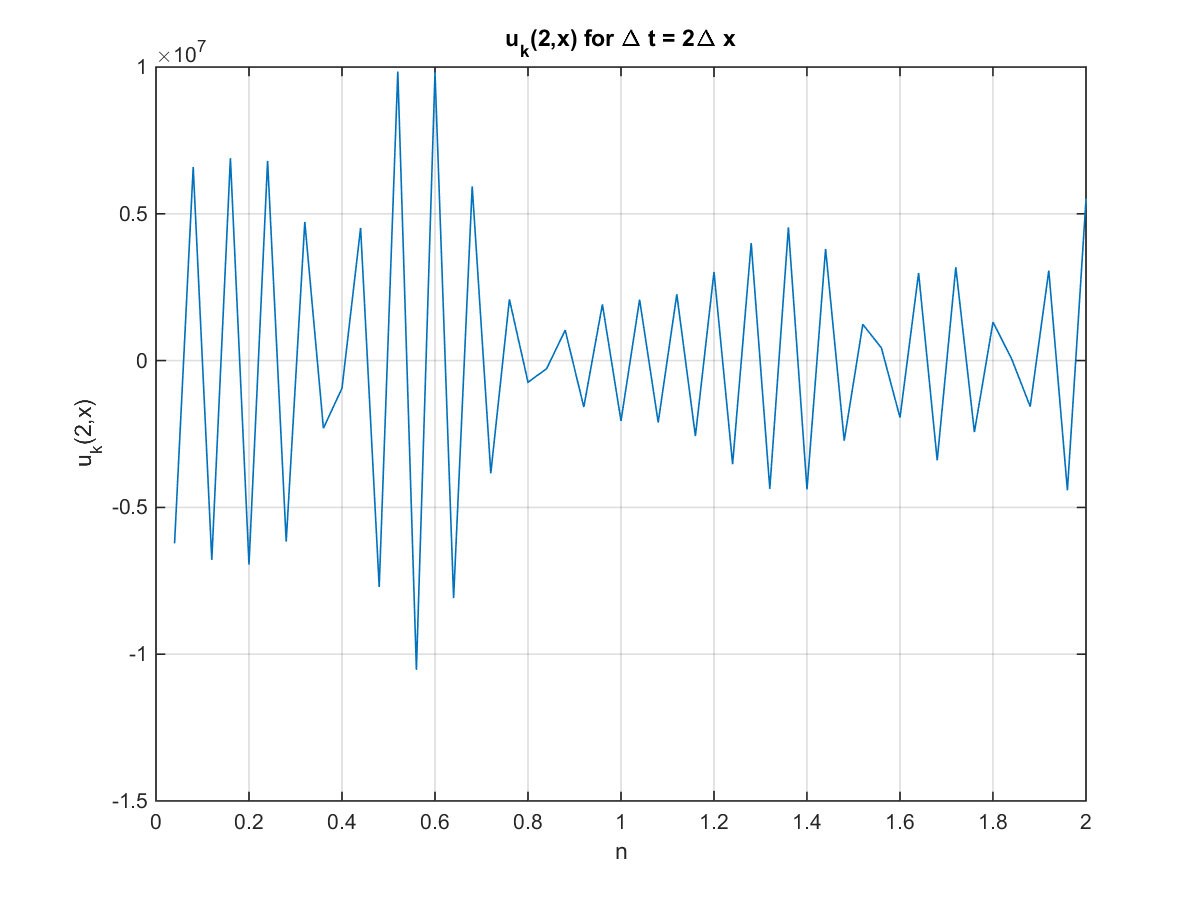
\includegraphics[scale=0.4]{hw6_4d1.png}
		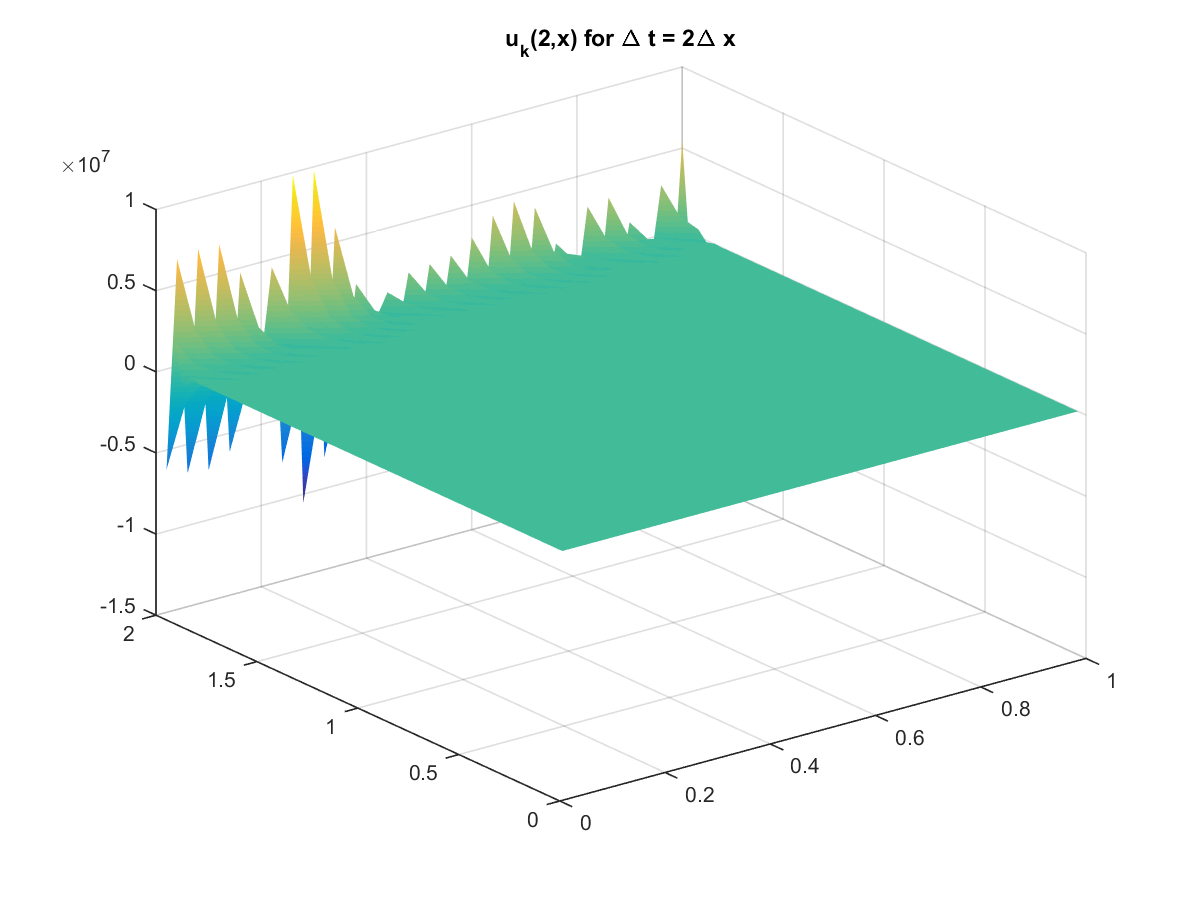
\includegraphics[scale=0.4]{hw6_4d2.png}
		\caption{$u_k(2,x)$ for $\Delta t = 2\Delta x$}
	\end{figure}
	- When $\Delta t$ is equal to the maximum: $\Delta t = \Delta x = 1/50$\\
	For $t = 2$, the step needed is $k = t/\Delta t = 2/(1/50) = 100$
	\begin{figure}[htp]
		\centering
		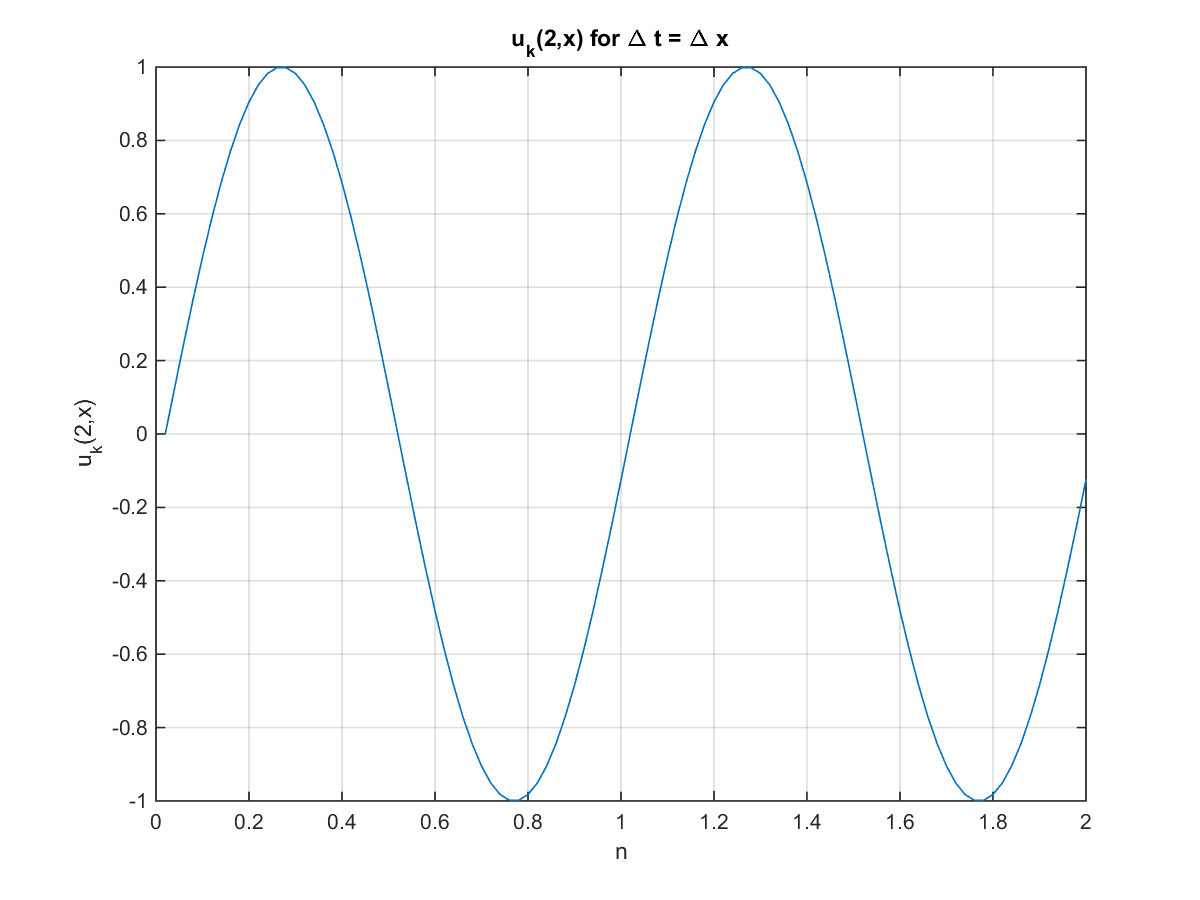
\includegraphics[scale=0.4]{hw6_4d3.png}
		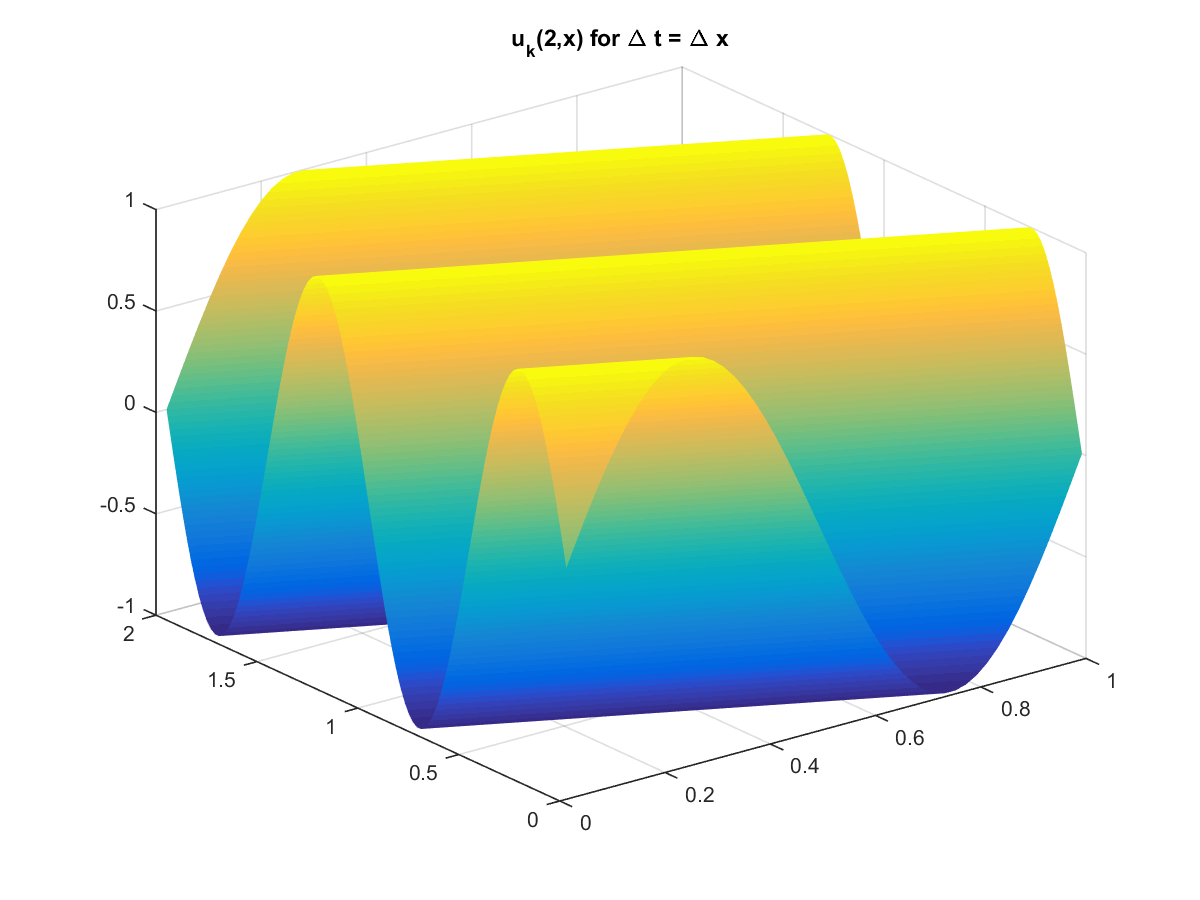
\includegraphics[scale=0.4]{hw6_4d4.png}
		\caption{$u_k(2,x)$ for $\Delta t = \Delta x$}
	\end{figure}
	
	\begin{lstlisting}
	n = 50; Dx = 1/n; x = 0:Dx:1; x(1) = [];
	A = -1*eye(n) + [zeros(n-1,1),eye(n-1); zeros(1,n)];
	A(n,1) = 1; A = A/Dx;
	
	% For Dt is twice time than the maximum value of Dx
	u1(:,1) = sin(2*pi*x); 
	Dt1 = 2*Dx; t1 = 0:Dt1:2; t1(1) = []; k1 = 2/Dt1;
	[T1,X1] = meshgrid(t1,x);
	for i =1:k1
		u1(:,i+1) = u1(:,i) + Dt1*A*u1(:,i);
	end
	u1(:,end) = [];
	figure; plot(t1,u1(:,end)); grid on;
	xlabel('n'); ylabel('u_k(2,x)');
	title('u_k(2,x) for \Delta t = 2\Delta x');
	print('hw6_4d1','-dpng');
	figure; surf(X1,T1,u1); shading interp;
	title('u_k(2,x) for \Delta t = 2\Delta x');
	print('hw6_4d2','-dpng');
	
	% For Dt is equal to the maximum value of Dx
	u2(:,1) = sin(2*pi*x);
	Dt2 = Dx; t2 = 0:Dt2:2; t2(1) = []; k2 = 2/Dt2;
	[T2,X2] = meshgrid(t2,x);
	for j =1:k2
	u2(:,j+1) = u2(:,j) + Dt2*A*u2(:,j);
	end
	u2(:,k2+1) = [];
	figure; plot(t2,u2(end,:)); grid on;
	xlabel('n'); ylabel('u_k(2,x)');
	title('u_k(2,x) for \Delta t = \Delta x');
	print('hw6_4d3','-dpng');
	figure; surf(X2,T2,u2); shading interp;
	title('u_k(2,x) for \Delta t = \Delta x');
	print('hw6_4d4','-dpng');
	
	\end{lstlisting}
\end{enumerate}
	
	



\end{document}